\subsection*{Velocity}
Det var �benlyst for os at vi i de forrige sprints have vurderet vores velocity for h�jt, s� i sprint 3 vurderede vi den ud fra hvor mange mandetimer vi havde n�et i sprint 2, minus lidt yderligere da vi faktisk havde lavet overarbejde i sprint 2. \\
F�lgende har vi fundet ud af vores velocity er lavere pga. manglende erfaring og teknisk niveau for nogle i gruppen.
Dette resulterer i at vi ikke helt har resourcerne for to hold men n�rmere 1,5.\\

Vi forventer at have 4 timer om dagen per mand i gruppen. Dvs. 6 mandetimer om dagen med 1,5 hold.\\

24 mande timer i en iteration\\
24*0,625 = 15 storypoints per uge\\
			3,75 storypoints per dag \\

\subsection*{Planl�gning}
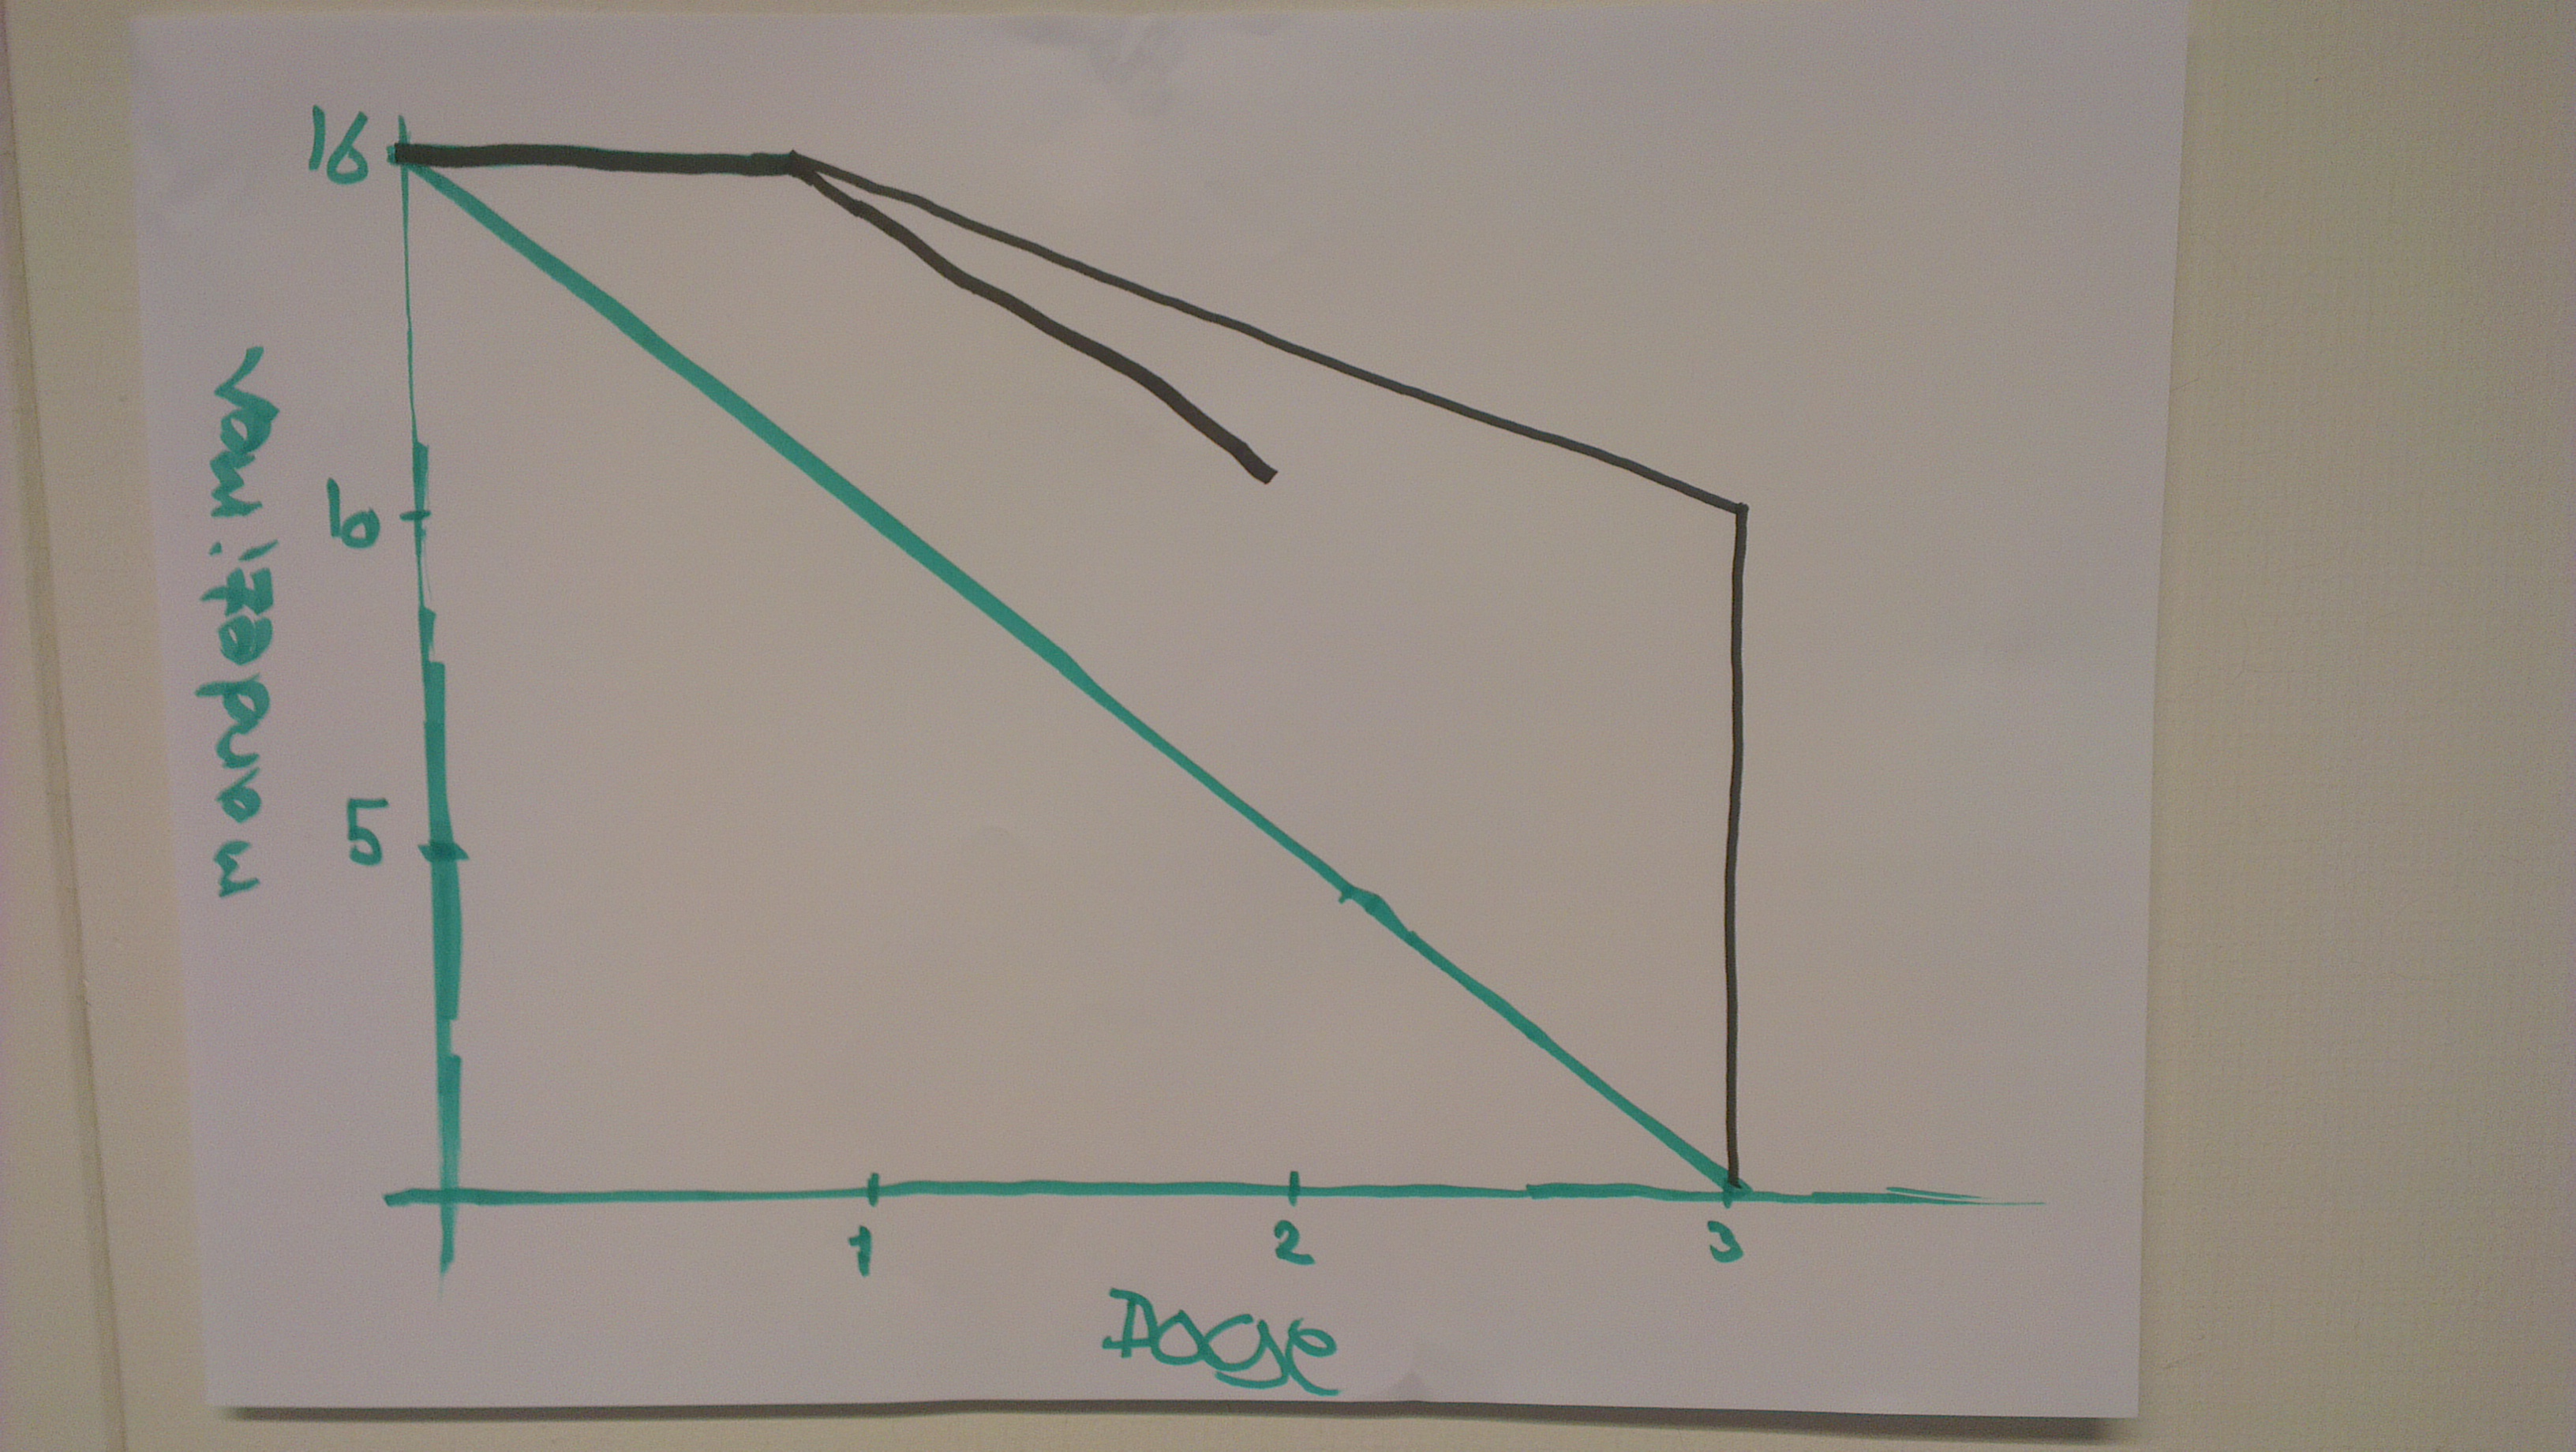
\includegraphics[scale=0.10]{includes/billeder/sprint3.jpg}

\subsubsection*{Product backlog}
Til product backloggen har vi i dette sprint tilf�jet en userstory med unit testing, samt at vi har �ndret prioriteten for diverse stories. \\
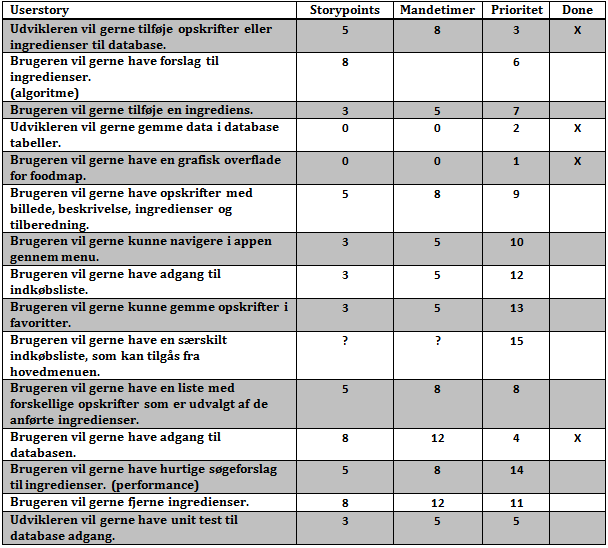
\includegraphics[scale=0.70]{includes/billeder/productbacklog_sprint3.png}

\subsubsection*{Sprint backlog}
I sprint backloggen for dette sprint indg�r de to userstories: \\
\begin{itemize}
\item Udvikleren vil gerne have unit test til database adgang.
\item Brugeren vil gerne have forslag til ingredienser. (algoritme)
\end{itemize}

Ud af disse to stories fik vi lavet unit testene.

\subsection*{Xp og scrum praktikker}
I sprint 3 benyttede vi fortsat XP praktikkerne: stand-up meeting, planning poker, par programmering, kollektivt kode ejerskab, kodestandarder, story board, metafor og simpelt design.

\subsection*{Produkt review}
Til reviewet viste vi vores foodmap gui med den funktionalitet vi havde n�et, samt vores unit test.

\subsubsection*{Konklusion af review}
N�ede kun unit testing.

\subsection*{Retrospektive}
\textsf{Hvad gik godt:} \\
Vi fik lavet unit test og dermed fik vi lidt mere kvalitetssikring ind over vores projekt. \\

\textsf{Hvad gik mindre godt}
Alt for kort sprint med de 3 mandedage og derfor for meget pres p� for at have noget klar til reviewet. Is�r iforhold til at have noget visuelt klar at kunne vise. \\
Vi havde lidt meget parprogrammering pga. vores fokus p� test. 

\textsf{Hvad �ndrer vi til n�ste sprint:} \\
Vi var sprint 3 det sidste sprint, men ellers havde vi prim�rt fors�ge at lave et l�ngere sprint hvor vi arbejdede lidt mere spredt.